\documentclass[a4paper,10pt]{article}
\usepackage[dvips]{color,graphicx}
\usepackage[dvips, bookmarks, colorlinks=false]{hyperref}


%opening
\title{Math508 Homework 12}
\author{Yu Huang}

\begin{document}

\maketitle

\begin{abstract}
Continuous state space Filtering
\end{abstract}

\section{Problem 3}
The difficult part is how to integrate the probability function. The idea is to replace the integral with a Riemann sum over the support where probability mass is not trivial. Based on the model, the signal $X_n$ is concentrated around 7 with small variance. As the sequence progresses, the general trend of $X_n$ goes upward though it's slow (due to the fact $X_{n+1} = 1.004X_n + 0.06X_nVn$).

\begin{equation}
\int_a^b f(x) dx = \sum_{x_i=a}^{x_i<b} f(x_i) \Delta x
\end{equation}


The support we pick is $[-20, 30]$. Different $\Delta x$ were tried. Smaller $\Delta x$, smaller mean squared error.


Figure~\ref{f1} is $\Delta x=0.15$. Figure~\ref{f2} is $\Delta x=0.34$. $\Delta x=0.5, 0.35$ could result in zero float division in normal density.

\begin{figure}
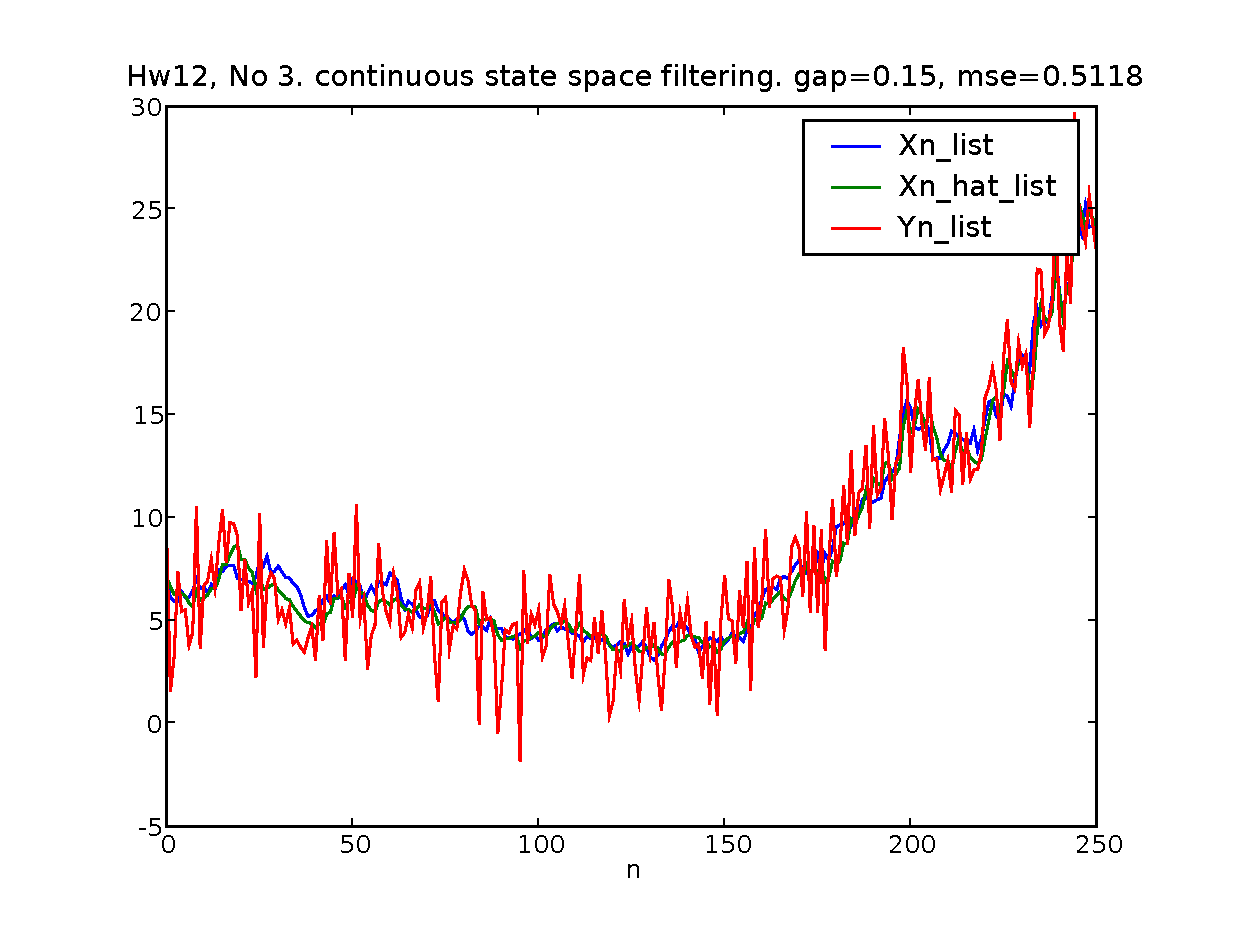
\includegraphics[width=1\textwidth]{hw12_3_gap_0_15.eps}
\caption{}\label{f1}
\end{figure}

\begin{figure}
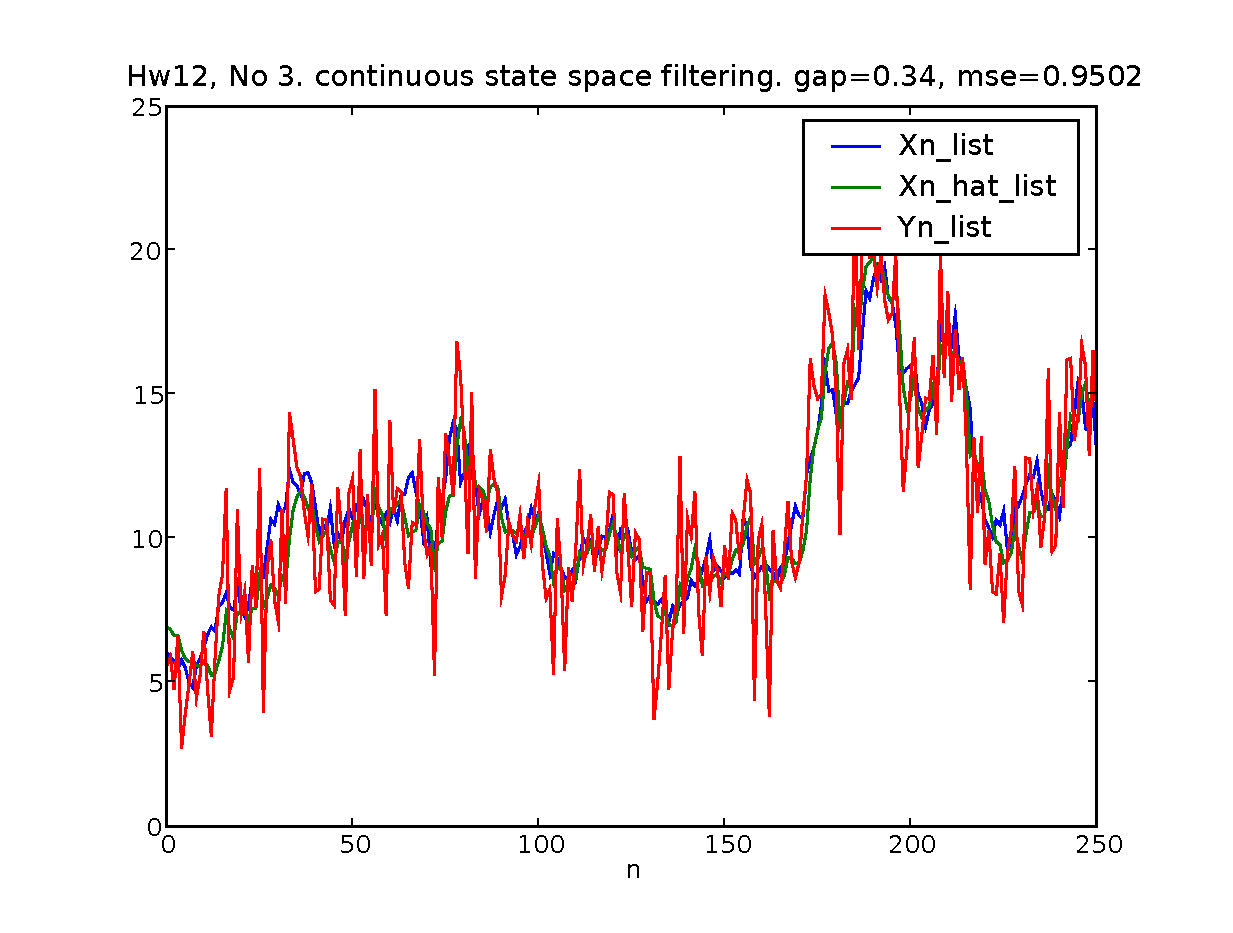
\includegraphics[width=1\textwidth]{hw12_3_gap_0_34.eps}
\caption{}\label{f2}
\end{figure}



\end{document}
